\chapter{Methods}
\label{ch:propalg}

本章將針對系統的各個流程進行深入的探討


\section{System architecture}
\label{sec:probdef}

本系統將翻譯原始句利用三個不同的線上翻譯系統取回翻譯假說,進一步利用了語言模型的分數決定了初步的最佳翻譯,之後再利用Substitution模組來取代錯誤翻譯的字,並進一步的利用Insertion模組將沒有被翻譯的字添補進來,最後則是利用Deletion模組將多餘的字刪除,\ref{fig:systemarchi}為本系統之系統架構圖。

\begin{figure}[tbh]
  \centering
  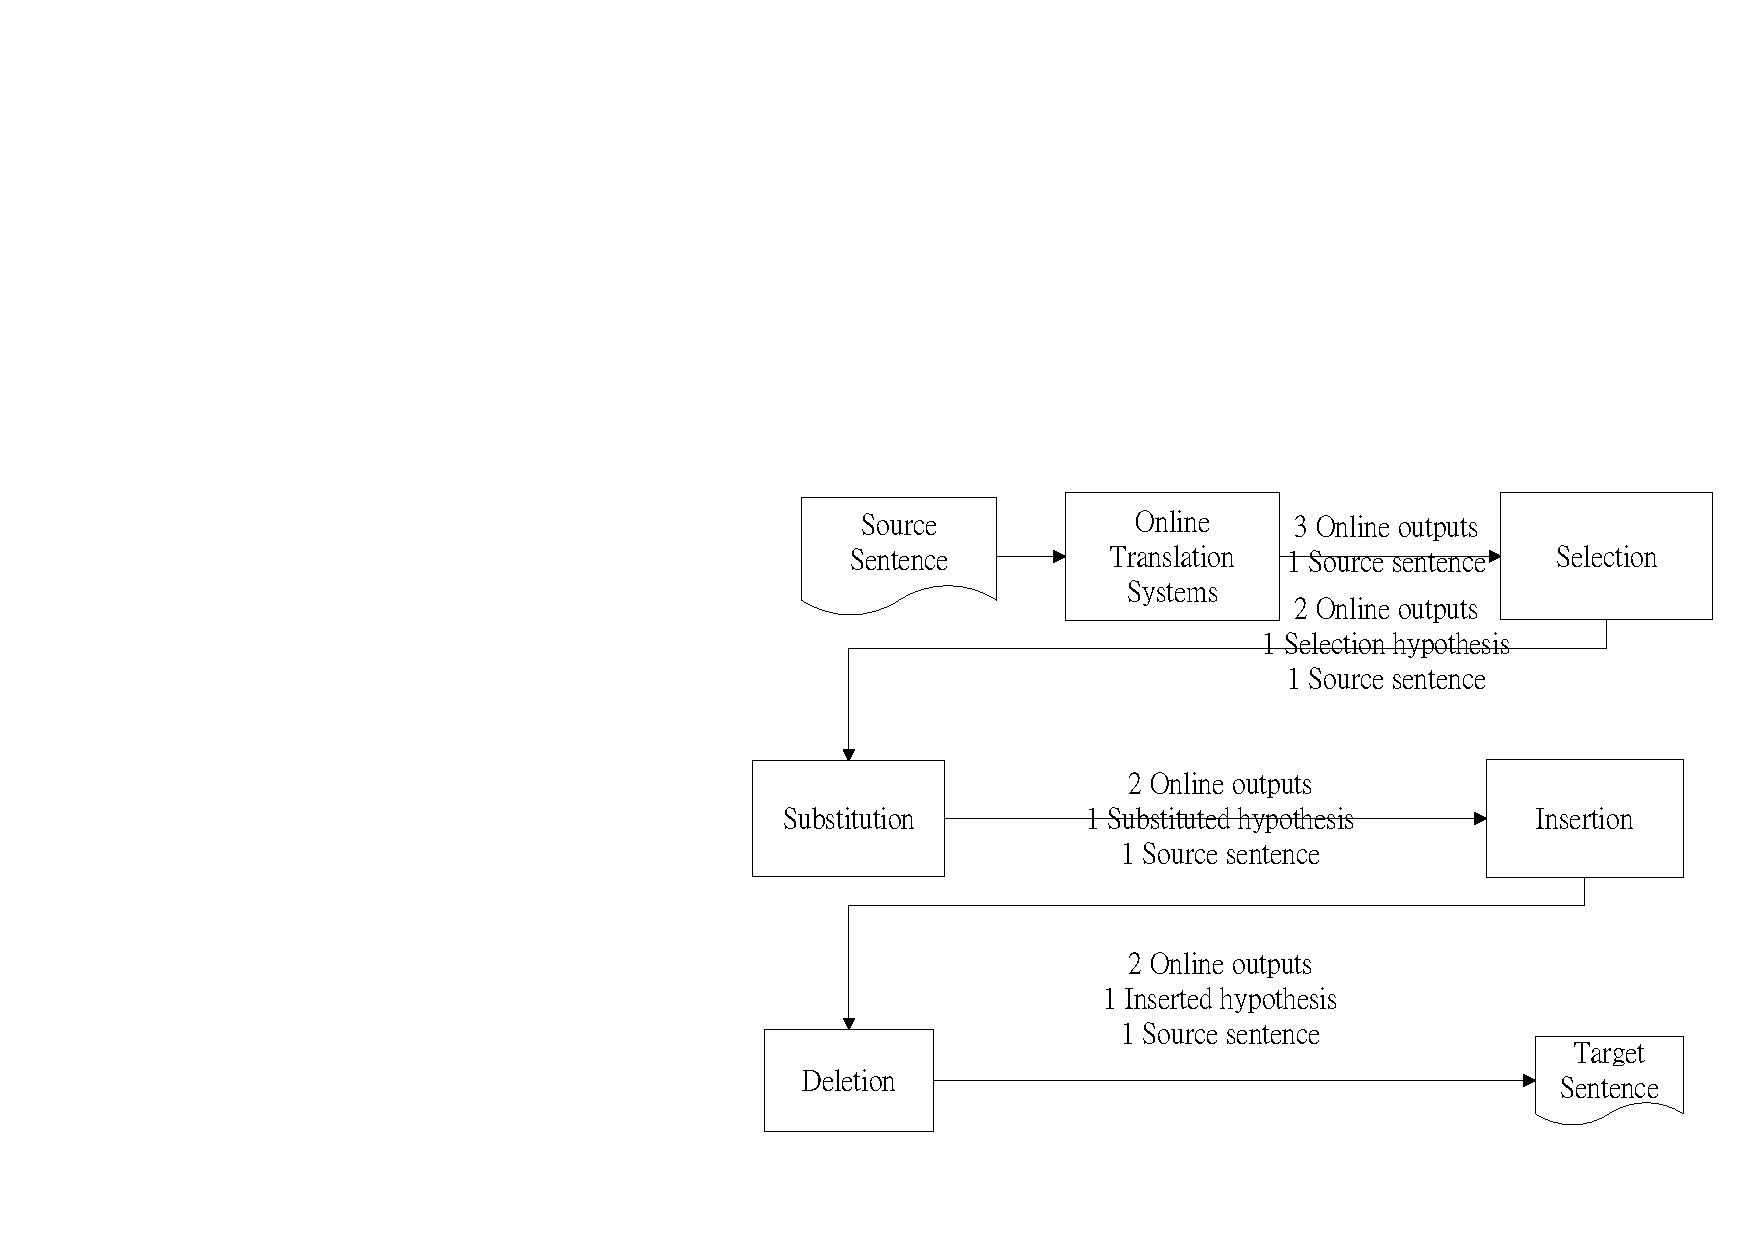
\includegraphics{figs/flow.pdf}
  \newcommand{\xc}{系統架構}
   \caption[\xc]{\xc.~\textcolor{magenta}}%%{Well, you are right. It looks
    %%  more like a placeholder than a figure showing the proposed
      %%algorithm.}}
  \label{fig:systemarchi}
\end{figure}


\subsection{Substitution}
\label{sec:Substitution}
本研究中利用SRILM\cite{stolcke2002sel}工具來訓練出一個5-gram的語言模型,而最佳的翻譯假說( $ E' $ )是根據以下選擇方法,針對top-one的假說來進行選擇。
\begin{equation}     
E' = \arg \mathop {\max }\limits_E \frac{1}{I}\sum\limits_{i = 1}^I {\log P(e_i |e_{i - 4}^{i - 1} )} 
  \label{eq:sel}
\end{equation}
$I$為各個翻譯假說的總長度,$e_i$為假說中的第$i$個字,$e_{i-4}^{i-1}$為$e_i$前面四個字,之所以後來會再以$\frac{1}{I}$對其Normalize,是考量到單純以語言模型分數來當作考量對長句子而言較顯不利,而Normalize過後的分數為各個字平均的分數,以此為基準下去比較,免除了長句不利的考量。
\subsection{Subection}
\label{sec:subection}
另外由於觀察發現,相同翻譯原始句所得到的翻譯假說中,同一個字出現在多個翻譯系統的翻譯假說中,則代表這個字為正確翻譯的機率較高,如果沒有出現在選擇的翻譯假說之中,則有可能是所選擇的翻譯假說沒有正確翻譯出來,因此給予一特定的門檻值,如果有超過半數的系統翻譯出相同的字($R$),而還擇的最佳翻譯假說中沒有出現該字,則考慮該字引入置換翻譯假說中字的可能性:


1.依照GIZA++所訓練出來雙向Translation table,考慮此字(替換字)所對應到翻譯原始句中的字($C_j$)(雙向機率最大者),而再由($C_j$)尋找其最有可能對應到翻譯假說中的字{$T_i$}。


2.比較$P(R|C_j)$以及$P(T_i|C_j)$彼此之間的機率大小,若$P(R|C_j) > P(T_i|C_j)$則考慮進行替換。


3.替換的評估如下:假設被替換字($T_i$)出現在翻譯假說中第$i$個位置,嘗試以替換字$R$代入後,考慮與翻譯假說中$i-1$位置的字($T_{i-1}$)及$i+1$位置的字($T_{i+1}$),利用Bigram的language model分數來進行比較,比較方式如下:


\begin{equation} 
	  h(x) = \left\{    
	    \begin{array}{ll}
     1         & \mbox{if} \log P(T_i|T_{i - 1})+\log P(T_{i + 1}|T_i) > \log P(R|T_{i - 1})+\log P(T_{i + 1}|R)\\
     0         & \mbox{otherwise}
    \end{array}
  \right.
  \label{eq:sub}
\end{equation}

4.若回傳結果為1則以替換字($R$)取代被替換字($T_i$)
\subsection{Insertion}
\label{sec:Insertion}

假使翻譯句已經包含了共同的翻譯字($R$)時,而($R$)位於其他翻譯假說($j$)之位置時,令$o_j$代表出現在其他假說中的$R$,考慮$o_j$與其前後各一個字($o_{j-1},o_{j+1}$)分別為片語的可能性,考慮將之引入翻譯假說中,詳細步驟如下:


1.找到$R$在最佳假說中的位置$i$,以$e_i$表示出現在最佳假說的$R$,計算以下機率考慮是否將$o_j$插入最佳假說中。

\begin{equation} 
	  h(x) = \left\{    
	    \begin{array}{ll}
1         & \mbox{if } {{\log P(o_{j - 1} |e_{i - 1} ) + \log P(e_i |o_{j - 1} )} \over 2} > \log P(e_i |e_{i - 1} )\\
0         & \mbox{otherwise}
    \end{array}
  \right.
  \label{eq:ins}
\end{equation}


2.若回傳結果為1則將$o_{i-1}$插入至最佳假說$i-1$的位置,若是回傳結果為0,則進一步考慮以$o_{i-1}$替換$e_{i-1}$的可能性,以下列式子判斷:

\begin{equation} 
	  h(x) = \left\{    
	    \begin{array}{ll}
1         & \mbox{if } {{\log P(o_{j - 1} |e_{i - 2} ) + \log P(e_i |o_{j - 1} )} \over 2} > {{\log P(e_{i - 1} |e_{i - 2} ) + \log P(e_i |e_{i - 1} )} \over 2} \\
0         & \mbox{otherwise}
    \end{array}
  \right.
  \label{eq:ins}
\end{equation}

3.若回傳結果為1則以$o_{j-1}$置換最佳假說中的$e_{i-1}$,若是回傳結果為0,則不進行任何動作。


4.同理以類似的方式考慮$o_{j+1}$引進的可能性。


\subsection{Deletion}
\label{sec:Deletion}

Deletion的步驟最主要是為了刪除假說中可能出現的錯誤翻譯,主要是參考